%\documentclass{beamer}
\documentclass[8pt]{beamer}
%\setbeamercolor{title}{fg=red!80!black,bg=red!20!white}
\definecolor{CEAColor}{rgb}{0.88, 0, 0.1} %
\usecolortheme[named=CEAColor]{structure}
\usepackage{tcolorbox}
\usepackage{graphicx,subcaption}
\usepackage{transparent}
%\usepackage{subfig}
%\usepackage{float}
%\usepackage{beamerthemesplit}
\graphicspath{{../img/}}
\setbeamertemplate{footline}[frame number]{}
\setbeamertemplate{navigation symbols}{}
\setbeamertemplate{footline}{}


\title{QUAD-BLOCKING}
\author{\tiny A.M. Vintescu$^{1}$}
\date{\today}
\begin{document}
%\frame{\titlepage}
%\section*{Outline}
%\frame{\tableofcontents}
\section{QUAD-BLOCKING}
\subsection{Programme Transversal de Comp\'{e}tences Simulation Num\'{e}rique}
\frame{
\vspace{-0.3cm}
\begin{minipage}[!T]{0.99\linewidth}
\begin{center}
\transparent{0.5} \textcolor{red}{\small \center{Programme Transversal de Comp\'{e}tences Simulation Num\'{e}rique}}
\vspace{-0.3cm}
\end{center}
\end{minipage}
\newline
\begin{minipage}[!T]{0.15\linewidth}

\includegraphics[width=0.98\linewidth]{logo_cea}
\end{minipage}
\begin{minipage}[!T]{0.84\linewidth}
\begin{minipage}[!T]{0.99\linewidth}
\begin{center}
\transparent{1.0} \normalsize \center{QUAD-BLOCKING}%: Automatic generation of block-structured quadrilateral meshes
%Automatic generation of block-structured quadrilateral \\ \medskip meshes: singularity graph extraction
\end{center}
\end{minipage}
\newline
\begin{minipage}[!T]{0.99\linewidth}
% Poster Authors 
\begin{center}
\scriptsize A.M. Vintescu$^{1}$, 
\scriptsize F. Ledoux$^{1}$,     
\scriptsize F. Kloss$^{2}$,
\scriptsize T. Fortuna$^{3}$,
\scriptsize V. Bergeaud$^{3}$\\
\end{center}
\end{minipage}
\newline
\begin{minipage}[!T]{0.99\linewidth}
\begin{center}
\tiny  $~^1$ CEA, DAM, DIF, Arpajon, France \hspace{2em}  
\tiny $~^2$ CEA, DEN, DM2S, Saclay, France \hspace{2em}  
\tiny $~^3$ CEA, DRT, LIST, Gif-sur-Yvette, France \hspace{2em}
\vspace{-0.3cm}
\end{center}
\end{minipage}
\end{minipage}
%\begin{minipage}[!T]{0.2\linewidth}
%
\includegraphics[scale=0.1]{logo_cea_list}
%\end{minipage}
\vspace{-0.1cm}
%\frametitle{List  displayedstep−by−step}
\begin{center}
\small Available: high-order method for fast simulations on quadrilaterals(2D)
\newline
\small $\rightarrow$ automatic generation of block-structured quadrilateral meshes
\newline
\vspace{-0.1cm}
\end{center}
\vspace{-0.1cm}
\captionsetup{labelformat=empty}
\vspace{-0.1cm}
\noindent
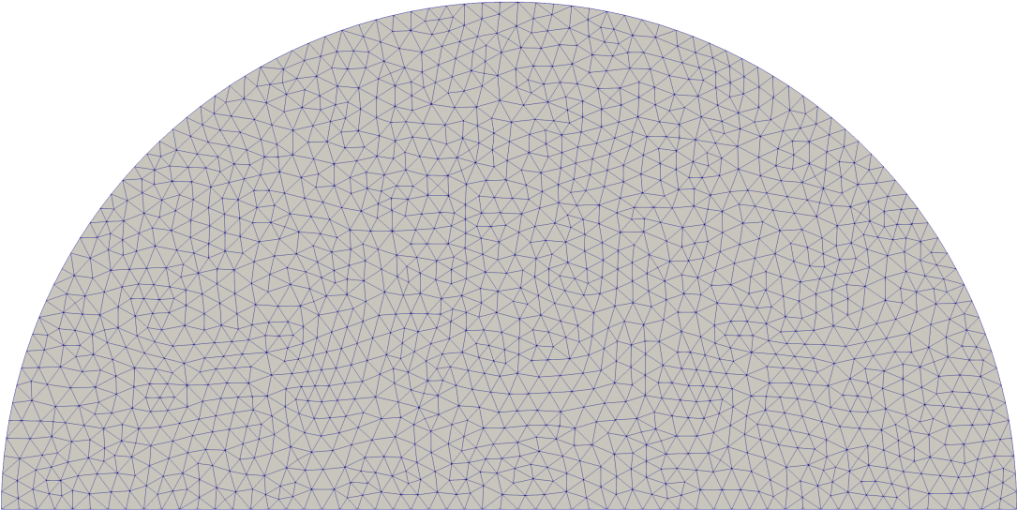
\includegraphics[width=0.24\linewidth]{1}
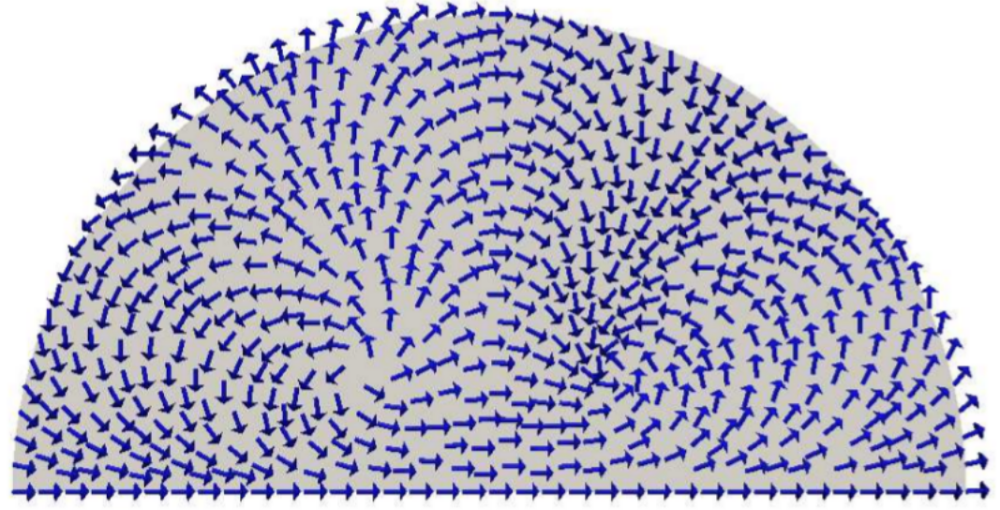
\includegraphics[width=0.24\linewidth]{2}
%-------------------------------------------------------------------------------------
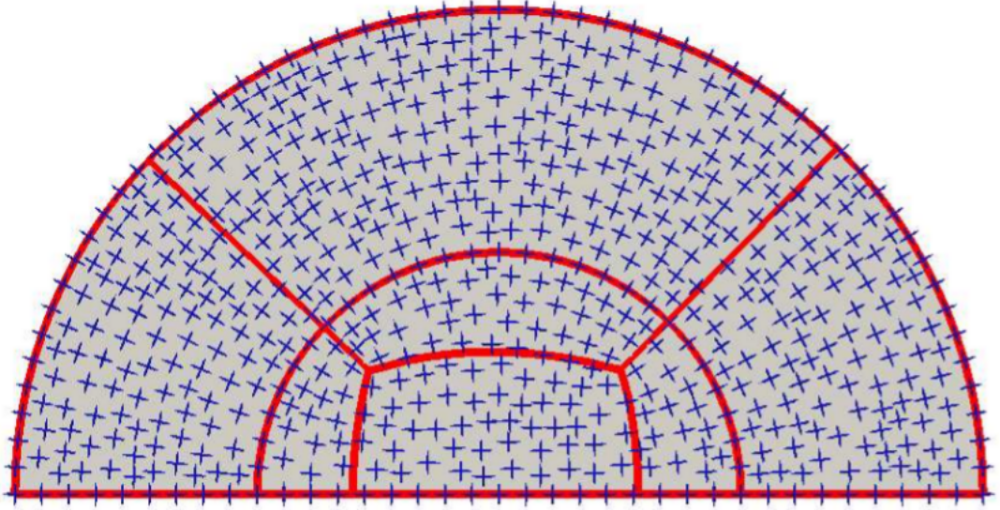
\includegraphics[width=0.24\linewidth]{3}
%\captionof{figure}{\textcolor{red}{\textbf{Singularity Graph Extraction}}}
%------------------------------------------------------------------------------------------------
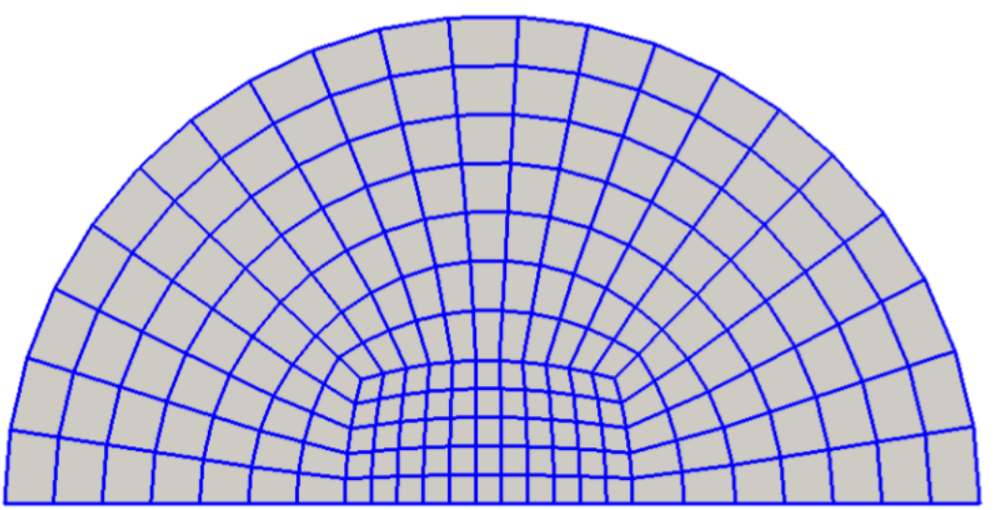
\includegraphics[width=0.24\linewidth]{4}
\newline
\begin{minipage}[!T]{1.0\linewidth}
\begin{center}
\textbf{Singularity Graph Extraction}
\end{center}
\end{minipage}
\newline
\begin{minipage}[!T]{1.0\linewidth}
\begin{minipage}[!T]{0.48\linewidth}
\begin{center}
\textbf{Continuous Strategy}
\newline
Challenges:
\newline
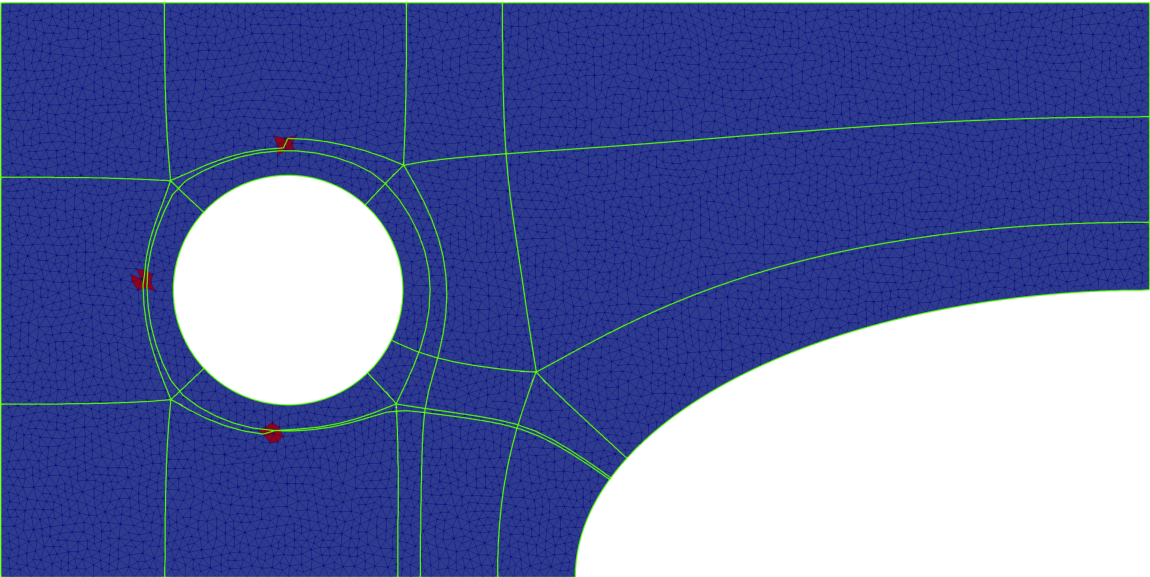
\includegraphics[width=0.5\textwidth]{HIS4-sim-Rad002}
\newline
%\captionof{figure}{\tiny }
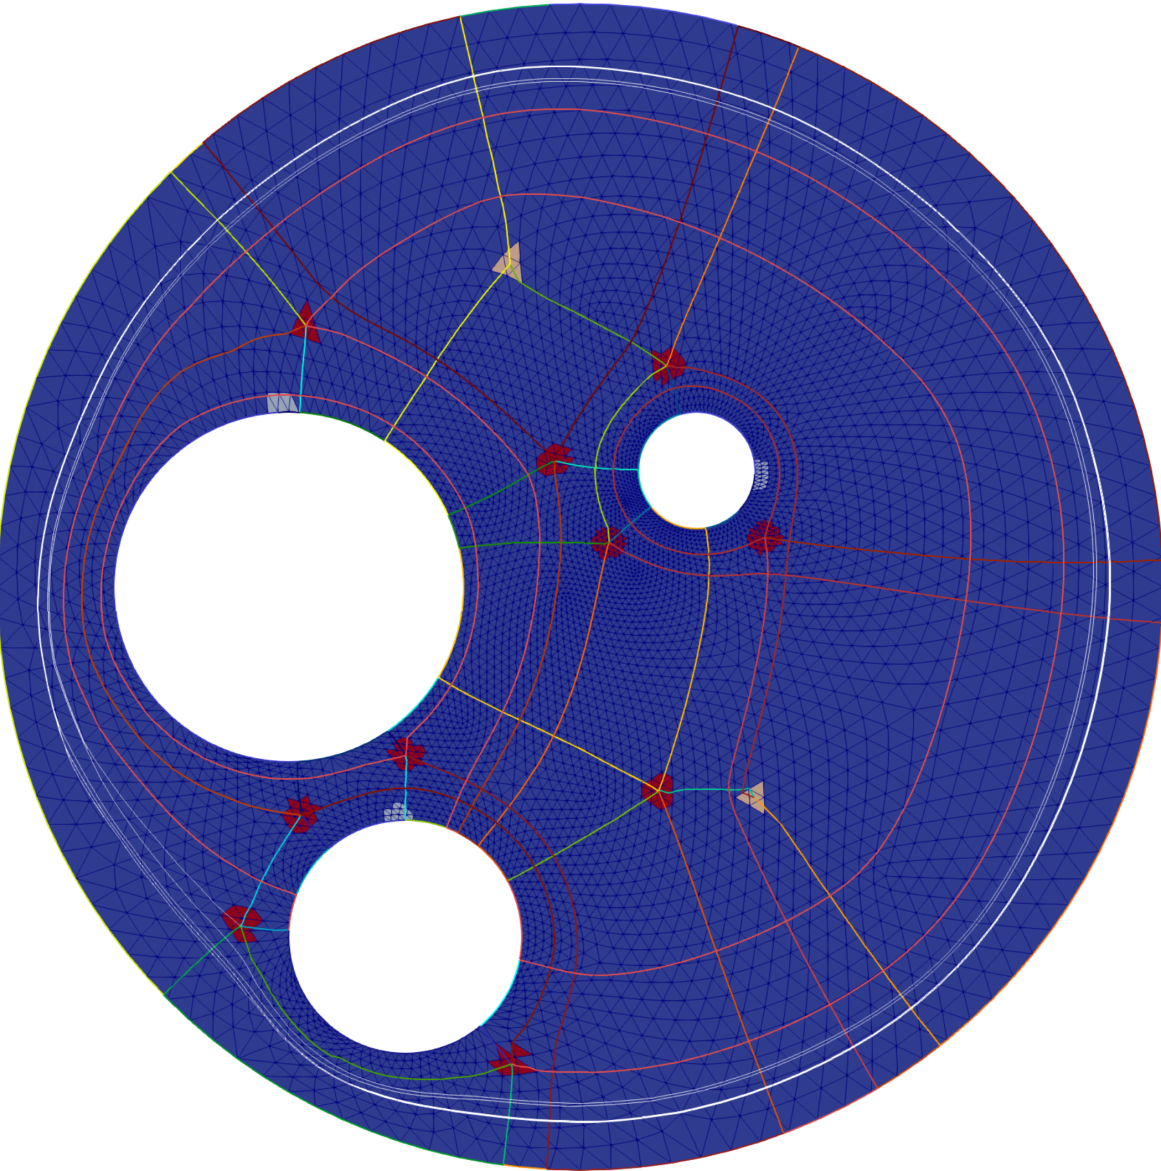
\includegraphics[width=0.4\textwidth]{Circle_with_circle_holes_refSS1-cycle}
%\captionof{figure}{\tiny }
%\newline
\begin{flushleft}
\tiny a) "miss the connection"
\newline
\tiny b) dependence on mesh resolution
\newline
\tiny c) dependence on proximity parameter
\newline
\tiny d) Cycles
\end{flushleft}
\end{center}
%\vspace{-0.3cm}
\end{minipage}
\begin{minipage}[!T]{0.48\linewidth}
\begin{center}
\textbf{Discrete Strategy}
\newline
Advantages:
\newline
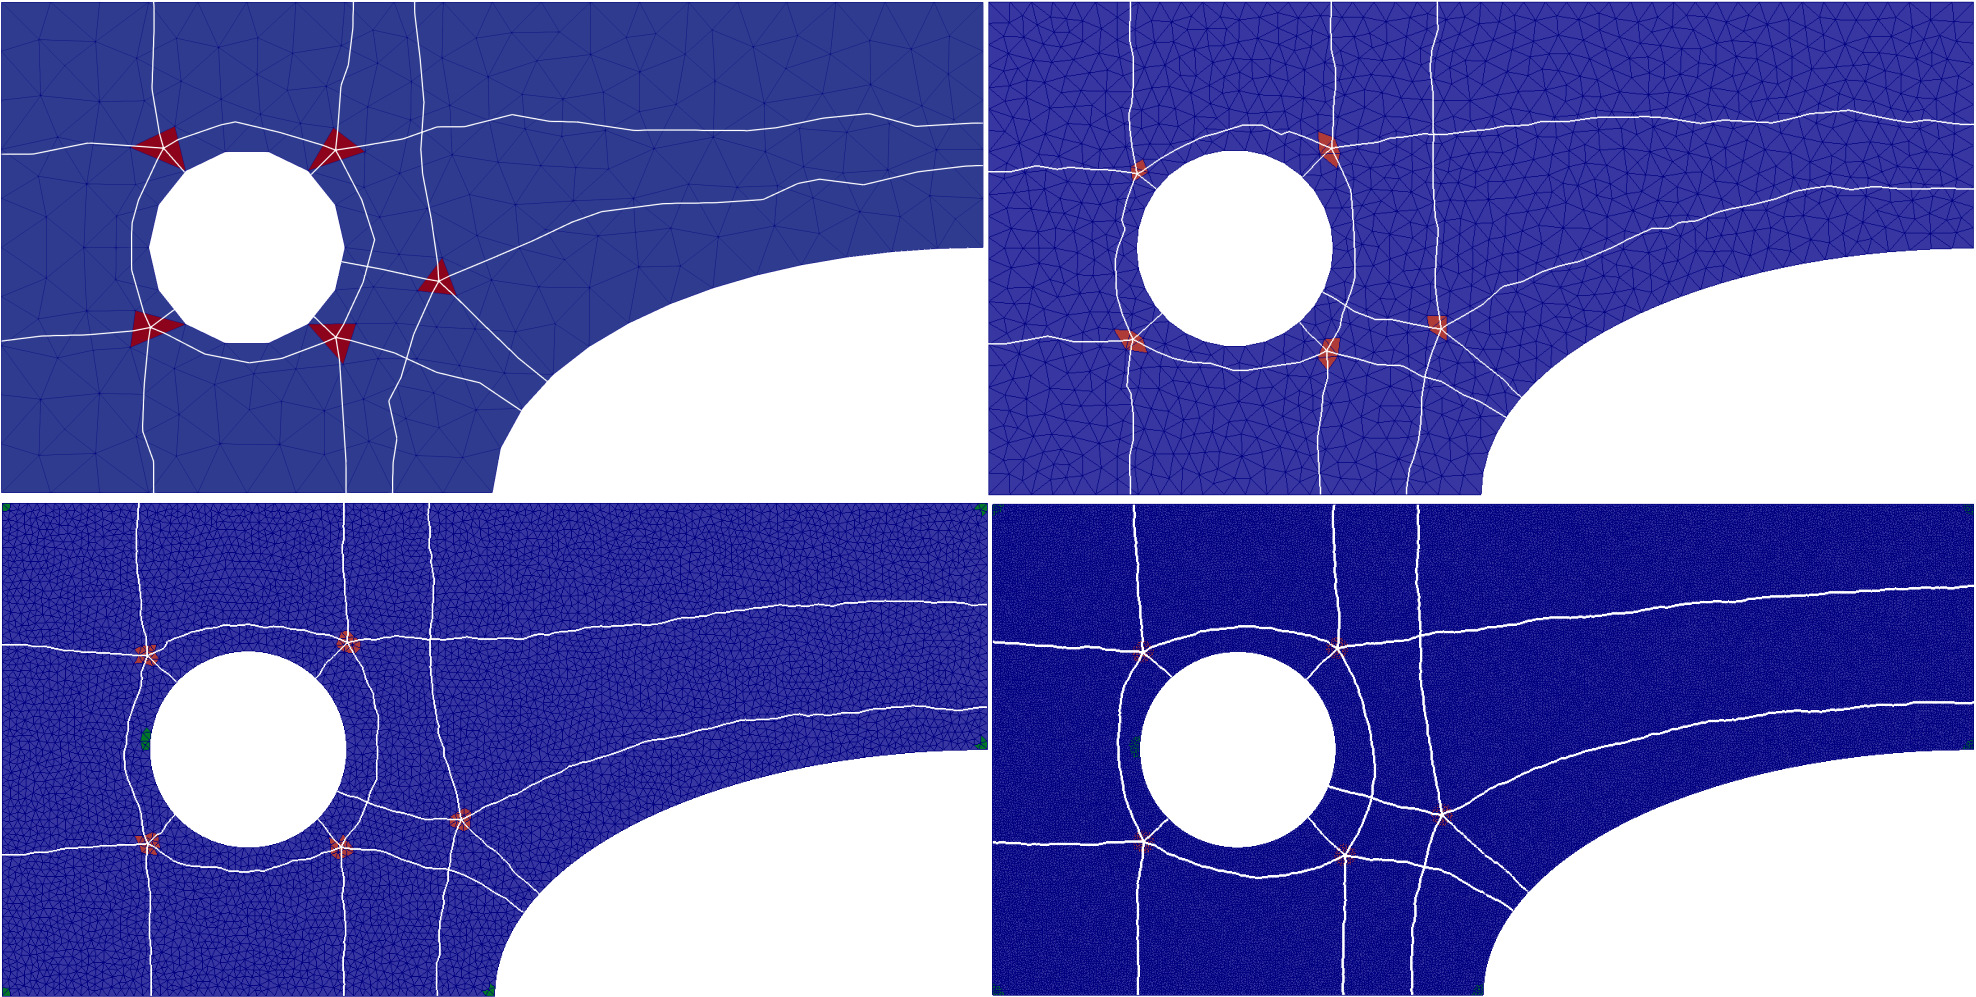
\includegraphics[width=0.95\textwidth]{HIS_collection}%\end{flushleft}
\newline
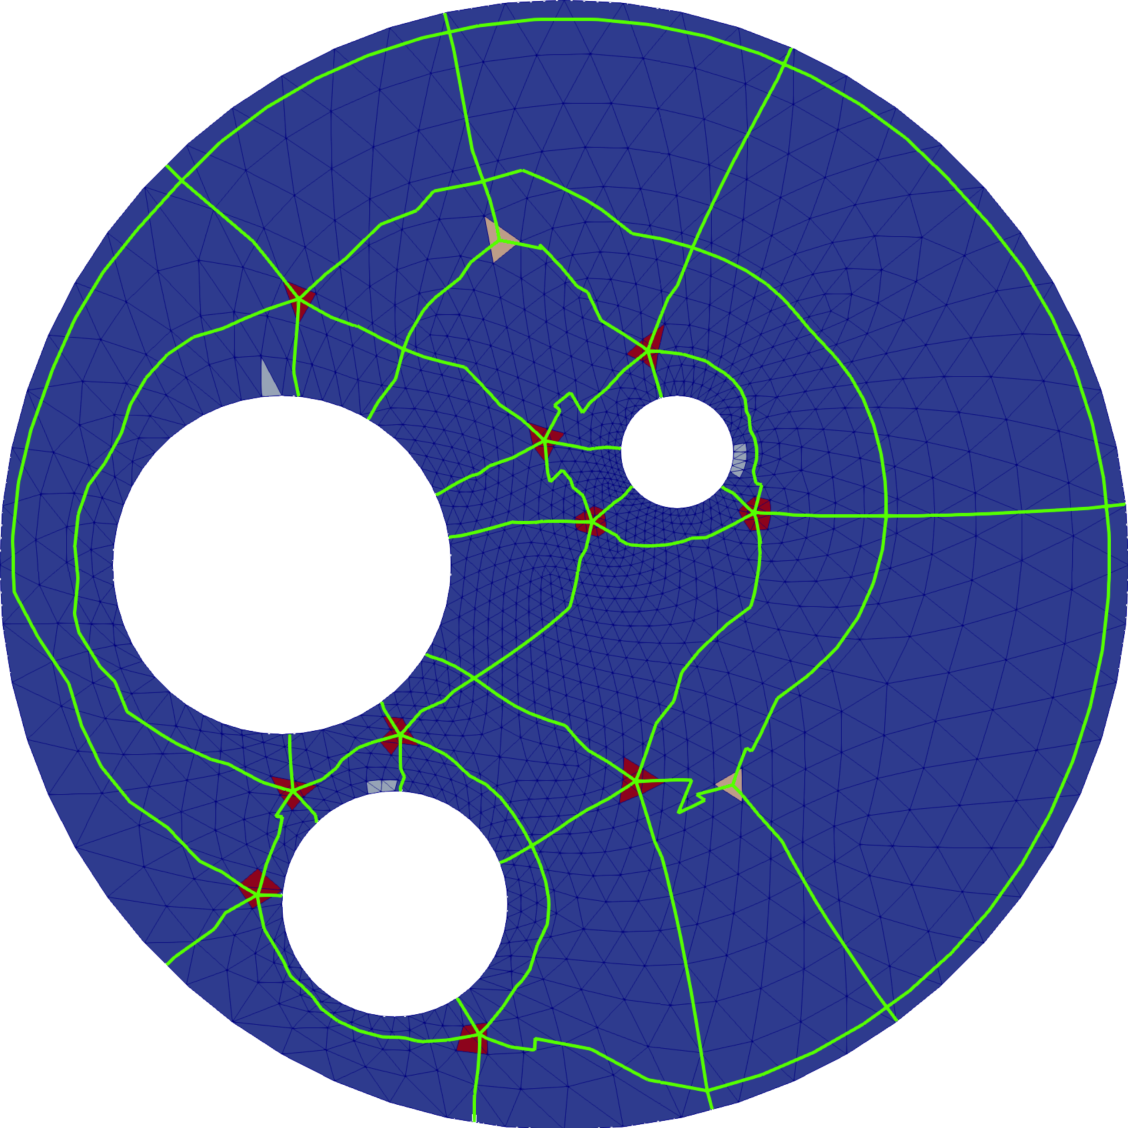
\includegraphics[width=0.4\textwidth]{CWCH_coarse-shortest_paths}
\end{center}
%\vspace{-0.3cm}
\end{minipage}
\end{minipage}
%\vspace{-6cm}
%\begin{minipage}[b]{1\linewidth}
%\vspace{-0.1cm}\noindent
%\begin{tcolorbox}[colframe=gray,boxrule=0.01pt,left=0mm,right=0mm,title=\Large $\ \ \ \ \ \ \ \ \ \ \ \ \ \ \ \ \ $Objectives $\ \ \ \ \ \ \ \ \ \ \ \ \ \ \ \ \ \ \ \ $Limitations$\ \ \ \ \ \ \ \ \ \ \ \ \ \ \ \ \ $]		%\begin{itemize}
%\vspace{-0.1cm}\noindent
%$\bullet$ Fully automatic method  $\ \ \ \ \ \ \ \ \ \ \ \ \ \bullet$  Dependence on input triangulation%	\item[$\bullet$] Fully automatic method
%\newline
%$\bullet$ High quality resulted quad blocks $\ \ \ \ \ \ \bullet$ Approximation errors%	\item[$\bullet$] High quality resulted quad blocks
%\vspace{-0.1cm}
%\end{tcolorbox}
%\end{minipage}
}
%\section{Current  A c t i v i t i e s}
%\subsection{ceva}
%\subsection{ceva}
%\section{Our Goals}
%\subsection{ceva}
%\subsection{ceva}
\end{document}